\chapter{Descrizione dell'algoritmo}
Il procedimento di pattern-matching sequenziale naive non sfrutta la possibile presenza di una serie di confronti con esito positivo (match), verificatasi prima di un esito negativo (mismatch) \footnote{esito positivo = corrispondenza di un carattere nel testo e un carattere nel pattern}.\\ Una conseguenza di tale approccio è la dipendenza del tempo di computazione sia dalla grandezza del testo($n$) che da quella del pattern alfanumerico ($m$), rendendo nel caso peggiore le prestazioni quadratiche rispetto ad $n$. Il numero di confronti effettuati, infatti, corrisponde a $\Theta ((n-m+1)m)$.\\
L'algoritmo utilizzato divide il testo in sezioni e ne assegna una ad ogni processore disponibile. Ognuno di questi, in parallelo rispetto agli altri, esegue una ricerca del pattern voluto con l'algoritmo KMP e restituisce l'indice della prima occorrenza trovata. Nel caso in cui il pattern sia presente all'interno del testo, verrà restituito l'indice minore tra quelli individuati dai processi; altrimenti ne verrà notificata l'assenza all'utente.
\section{Algoritmo Knuth Morris Pratt}\label{KMP}
L'algoritmo KMP esegue pattern-matching in tempo lineare rispetto alla sola dimensione del testo. 
Sfrutta i risultati ottenuti in precedenza per evitare di dover effettuare nuovamente confronti su caratteri già analizzati. Per rispettare queste prestazioni viene eseguita inizialmente una fase di pre-processamento del pattern, utilizzata per evitare di dover compiere maggiori confronti come nel procedimento naive\cite{func}.\\ Per comprendere in che modo venga effettuata questa fase, è conveniente introdurre i concetti di prefisso e suffisso di una stringa.
Con il termine {\itshape prefisso} di lunghezza $k$  di una stringa si intendono i primi $k$ caratteri che la compongono, mentre con {\itshape suffisso} di lunghezza $k$ gli ultimi $k$.
Per ogni prefisso del pattern, viene ricercato il suo prefisso di lunghezza maggiore, che ne costituisca anche un suffisso. Il pre-processamento restituisce un vettore di numeri interi della stessa lunghezza del pattern, chiamato vettore di fallimento o fail vector. Questo contiene, in ogni cella di indice $j$, la lunghezza del prefisso ricercato, come specificato in precedenza, nella sottostringa del pattern (che si estende dal primo carattere al $j$-esimo) (Figura \ref{esempio_fail}). In questo modo, accedendo ai valori salvati nel vettore, nel caso in cui si verifichi un mismatch, si potrà sapere quali caratteri confrontare successivamente all'interno del testo e del pattern.
\begin{figure}[h]
\centering
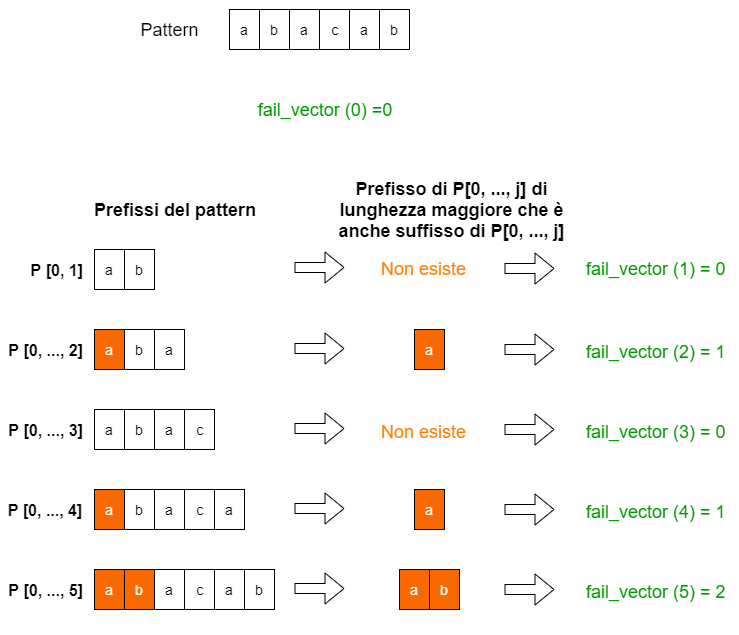
\includegraphics[scale=0.6, angle=0]{./Images/Chapters/Esempio_Fail}
\caption{\footnotesize{Esempio di computazione del fail vector per il pattern "abacab".}}
\label{esempio_fail}
\end{figure}
Una volta terminata la computazione del vettore, l'algoritmo inizia a confrontare gli elementi del testo con quelli che formano il pattern cercato. Nel caso in cui si verifichi un mismatch tra l'elemento $i$-esimo del testo e il $j$-esimo del pattern, il successivo confronto avviene tra l'elemento $t$-esimo del testo e l'elemento $k$-esimo del pattern. Gli indici $t$ e $k$  vengono calcolati con la seguente regola: 
$$
\bigg\{
\begin{array}{llcl}
{k=fail\_vector[j-1]} & {t=i} & {\:\:\:\:} & {se\:j\ne 0} \\
{k=0} & {t=i+1} & {\:\:\:\:} & {se\:j = 0} \\
\end{array}
$$
Una volta che i confronti hanno esito positivo per ogni carattere del pattern viene restituito l'indice iniziale dell'occorrenza del pattern nel testo.\\ \\

\section{Parallelizzazione}\label{Parallel}
Sfruttando più processori è possibile effettuare la ricerca del pattern in più porzioni del testo contemporaneamente. In fase di esecuzione, il programma riceve in input da linea di comando il nome del file contenente il testo e il pattern da cercare. \\ Per prima cosa viene selezionato un processore che funga da "master" e si occupi di elaborare tutte le informazioni necessarie per l'esecuzione dell'algoritmo KMP. Nel nostro caso questo processore "privilegiato" è quello di rank 0 e i suoi compiti principali sono:
\begin{enumerate}

\item{\textbf{Pre-processamento del pattern}\\
Calcola il fail vector applicando al pattern di partenza la funzione di fallimento
}
\item{\textbf{Elaborazione del testo}
Legge in input il nome del file in cui cercare il pattern e si occupa di aprire lo stream verso di esso. Legge il contenuto del testo ed in seguito chiude lo stream verso di esso. Elabora le stringhe necessarie agli altri processori per applicare il KMP attraverso due fasi (Figura \ref{esempio_ciclo}):
\begin{itemize}
\item{\textbf{Ciclo 1}\\
Una volta salvato l'intero testo all'interno di una stringa, rimuove $m-1$ elementi da essa ( $m$ = lunghezza del pattern) e la divide in un numero di sezioni pari al numero di processi disponibili.\\Se la stringa risultante dalla rimozione degli ultimi caratteri non dovesse essere un multiplo del numero di processori utilizzati, viene svolta una ripartizione intera della stringa e gli elementi non inclusi vengono inviati al processore di $rank=numero_processori-1$. La cosa più importante è che le stringhe debbano essere inviate rispettando l'ordine crescente dei rank e associandole in questo modo ai vari processori.
}
\item{\textbf{Ciclo 2}\\
Nel caso in cui siano presenti occorrenze del pattern a cavallo tra due sezioni del testo, calcolate nel \textbf{Ciclo 1}, non verranno rilevate. Per risolvere tale problema, il processore $0$, elabora anche le sottostringhe necessarie a ciascun processore per verificare la presenza di possibili occorrenze in quelle zone.\\Le sequenze elaborate in questa fase sono costituite dagli ultimi $m-1$ caratteri di una sezione del \textbf{Ciclo 1} e i successivi $m-1$ caratteri. Da questa elaborazione del testo, si può evincere la nostra scelta di escludere alcuni caratteri nel primo ciclo.
\begin{figure}[h]
\centering
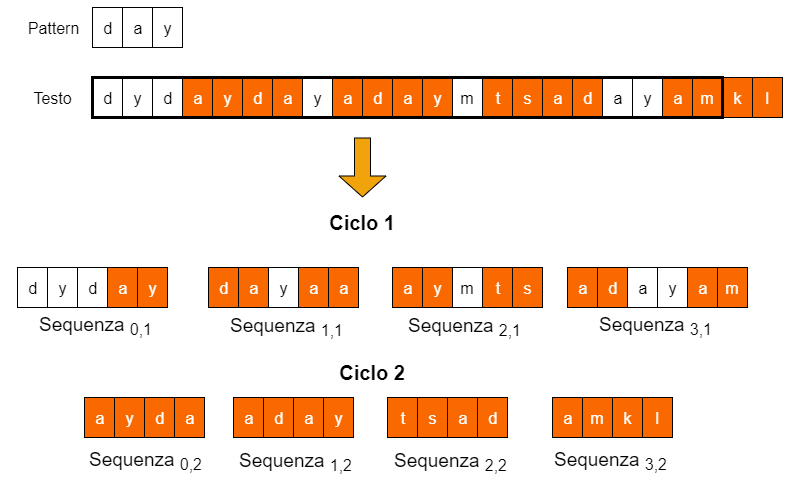
\includegraphics[scale=0.6, angle=0]{./Images/Chapters/Esempio_Ciclo}
\caption{\footnotesize{Esempio di computazione delle sequenze dei Cicli 1  e 2, utilizzando 4 processori.}}
\label{esempio_ciclo}
\end{figure}
}
\end{itemize}
}
\item{\textbf{Distribuzione dei dati}
Distribuisce a ogni processore le sottostringhe elaborate nel \textbf{Ciclo 1} e nel \textbf{Ciclo 2} ed il fail vector calcolato nella prima fase. Inoltre invia ad ogni processore il valore intero necessario per stabilire quale sia l'indice di un'eventuale occorrenza nelle stringhe del Ciclo 2, all'interno del testo originario. 
}
\item{\textbf{Gestione dell'output}
Verifica quale sia l'indice minore tra quelli restituiti da ogni processore e mostra sullo standard output. Nel caso in cui non sia stato trovato il pattern, notifica ciò all'utente.
}
\end{enumerate}

Tutti i processi, compreso il "master", in seguito alla distribuzione dei dati da parte del processore di rank 0, applicano l'algoritmo KMP sulle stringhe del Ciclo 1. Nel caso in cui non trovassero un'occorrenza, eseguono la stessa ricerca sulla stringhe del Ciclo 2. I risultati vengono poi inviati verso il "master" che effettuerà la gestione dell'output.